\documentclass[12pt,twoside]{article}

\usepackage{hyperref}
\usepackage{amsmath}
\usepackage{amsfonts}
\usepackage{amssymb}
\usepackage{amsthm}
%\usepackage{palatino,lettrine}
\usepackage{fancyhdr}
\usepackage{epsfig}
\usepackage[round,comma,sort]{natbib}
\usepackage{simplemargins}
\usepackage{setspace}
\usepackage{supertabular}
\usepackage{graphicx}
\usepackage{booktabs}
\usepackage[margin=1.5cm]{caption}



\newcommand{\profs}{Prof. Jeffrey Varner}
\newcommand{\subj}{1120}

\newlength{\toppush}
\setlength{\toppush}{2\headheight}
\addtolength{\toppush}{\headsep}

\newcommand{\htitle}[3]{\noindent\vspace*{-\toppush}\newline\parbox{6.5in}
{\textit{Introduction to Chemical Engineering: ENGRI 1120}\hfill\newline
Chemical and Biomolecular Engineering, Cornell University \hfill #3\newline
%\profs\hfill Handout #1\vspace*{-.5ex}\newline
\mbox{}\hrulefill\mbox{}}\vspace*{1ex}\mbox{}\newline
\begin{center}{\Large\bf #2}\end{center}}

\newcommand{\handout}[3]{\thispagestyle{empty}
 \markboth{ENGRI 1120 #2}{ENGRI 1120 #2}
 \pagestyle{myheadings}\htitle{#1}{#2}{#3}}

%\setlength{\oddsidemargin}{0pt}
%\setlength{\evensidemargin}{0pt}
%\setlength{\textwidth}{6.5in}
%\setlength{\topmargin}{0in}
%\setlength{\textheight}{8.5in}

%\doublespace
\onehalfspace
\setallmargins{1in}

\renewcommand{\rmdefault}{phv}\renewcommand{\sfdefault}{phv}
\captionsetup[figure]{font=small,labelfont=small}

\begin{document}


\handout{1}{PRACTICE PRELIM 2}{F2022}
\setlength{\parindent}{0pt}

% \newcommand{\solution}{
%   \medskip
%   {\bf Solution:}
% }

\medskip
\hrulefill
\medskip

\vspace{0.25in}

VERSION: DELTA-2

\vspace{0.25in}

NAME:

\vspace{0.25in}

\medskip
\hrulefill
\medskip

\begin{enumerate}

  \item{Prelim 2 has \textit{two} problems and is worth a total of XX points.}
  \item{You may use your course notes (on the computer, iPad, etc., or paper) or other course materials, e.g., discussion problems, to formulate your solutions.}
  \item{Do not consult with any other person regarding the prelim (except the TAs or JV),
  or use \textit{any form of electronic communication} to discuss the prelim questions.
  Violation of this policy will result in a ZERO for the prelim.}
  \item{Do not consult the interwebs to search for the prelim questions/solutions.
  Violation of this policy will result in a ZERO for the prelim.}
  \item{Show your work and state all assumptions or simplifications.}
  \item{Good luck!}

\end{enumerate}

\medskip
\hrulefill
\medskip



\begin{enumerate}


% Question 2 ===================== %
\clearpage
\begin{figure*}[h!]\centering
    \captionsetup{width=0.75\linewidth}
    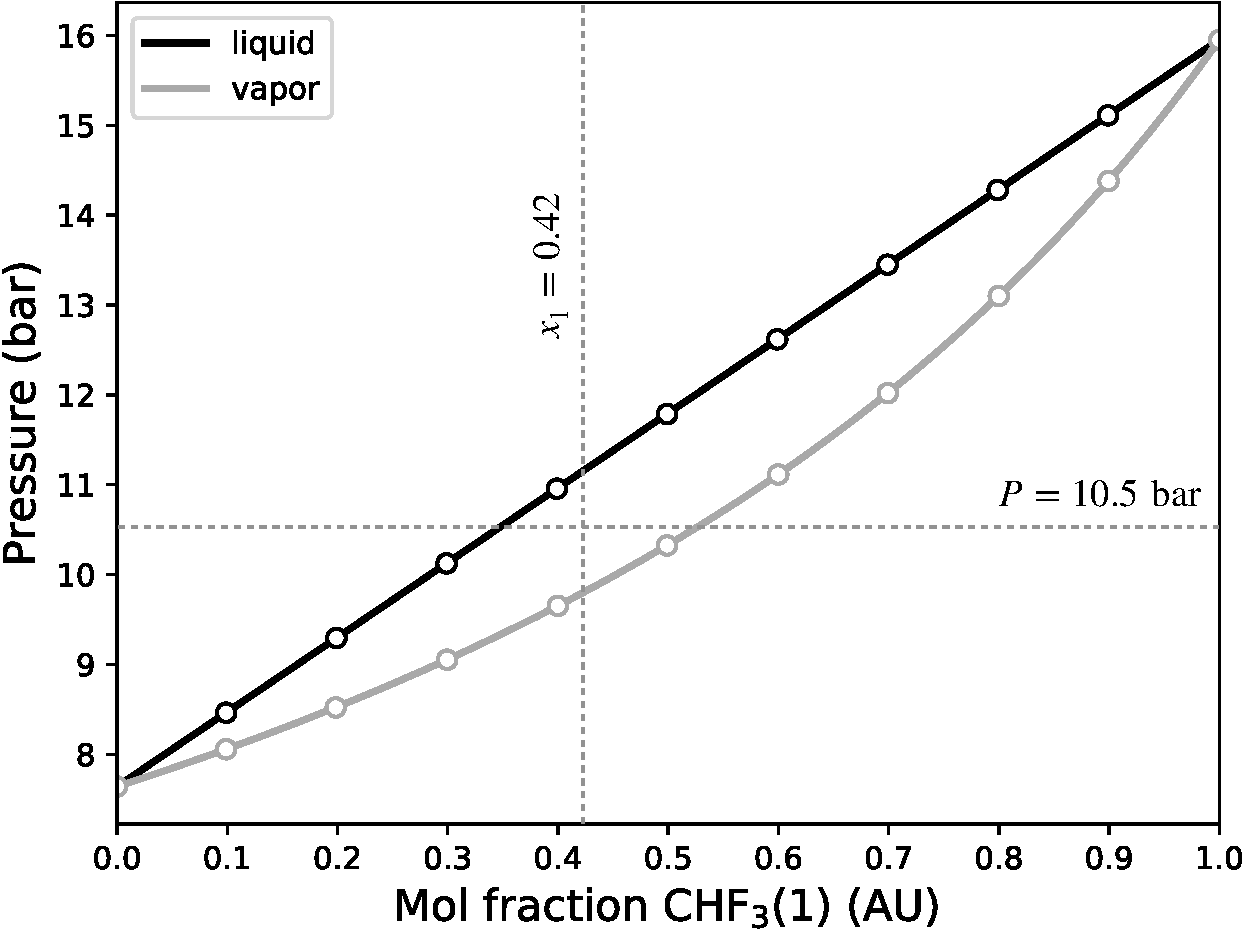
\includegraphics[width=0.75\textwidth]{./figs/VLE-Ideal-Pxy-P2-F19.pdf}
    \caption{Pressure (bar) versus composition (x$_{1}$ and y$_{1}$) for a binary mixture of CHF$_{\mathrm{3}}$(1)/C$_{\mathrm{2}}$F$_{\mathrm{6}}$(2) computed assuming ideal liquid and vapor phases.}\label{fig-VLE-ideal-problem}
    \end{figure*}
    
    \item{(XX points) Cornell Inc. was hired to design a flash separation process for a binary ($\mathcal{M}$ = 2) mixture of CHF$_{\mathrm{3}}$(1)/C$_{\mathrm{2}}$F$_{\mathrm{6}}$(2).
    The engineering team performed initial design calculations using Raoult's law for z$_{1}$ = 0.42
    (Fig. \ref{fig-VLE-ideal-problem}). Let the saturation pressure of component $i$ be described by the
    Antoine equation:
    \begin{equation}
      \log_{10}\left(P_{i}^{sat}~[\mathrm{bar}]\right) = A - \frac{B}{C+T[K]}
    \end{equation}where the Antoine parameters are given by:
    
    \begin{table}[!ht]
      \centering
      \caption{Antoine parameters for the Flash problem.}
      \setlength{\tabcolsep}{18pt}
      \begin{tabular}{c|c|c|c}\toprule
        Species & A & B & C \\ \toprule
        CHF$_{\mathrm{3}}$ & 4.45 & 718.1 & -22.01 \\
        C$_{\mathrm{2}}$F$_{\mathrm{6}}$ & 3.980 & 677.1 & -24.51 \\\bottomrule
      \end{tabular}
    \end{table}
    
    \textbf{Assumptions}: (i) the Flash drum operates at steady-state;
    (ii) vapor-liquid equilibrium occurs everywhere inside the drum at some (T,P);
    (iii) treat both the vapor and liquid phases as ideal;
    (iv) the Flash drum is well-mixed;
    (v) a single liquid feed (stream 1) enters, and a vapor (stream 2) and liquid (stream 3) exit the drum;
    (vi) R = 8.314$\times$10$^{-2}$ L bar K$^{-1}$ mol$^{-1}$.
    
    \begin{itemize}
      \item[a)]{(XX points)~What temperature T (K) is the Flash drum operating at? (place your estimated T in Table
      \ref{tbl-state-flash-problem}).}
      \item[b)]{(XX points)~\textit{Graphically} estimate the mising values in Table \ref{tbl-state-flash-problem} assuming the Flash drum operates at P = 10.5 bar with a input feed rate of $\dot{F}$ = 10 mol/t and $z_{1}$ = 0.42.}
      \item[c)]{(XX points)~\textit{Analytically} check the graphical estimates of $\dot{L}$ and $\dot{V}$ using the pressure summation expression:
      \begin{equation}
        \sum_{i\in\mathcal{M}}z_{i}\left[\frac{P_{i}^{sat}}{P}\left(\frac{\dot{V}}{\dot{F}}\right)+\frac{\dot{L}}{\dot{F}}\right]^{-1} = 1
      \end{equation} If this expression is \textit{significantly} different than 1 (greater than $\pm$~10\% difference),
      please re-estimate your values (show your work).}
    \end{itemize}
    
    \clearpage
    
    \begin{table}[!ht]
      \centering
      \caption{State table for the Flash problem.}\label{tbl-state-flash-problem}
      \renewcommand{\arraystretch}{2.0}
      \setlength{\tabcolsep}{18pt}
      \begin{tabular}{c|c|c|c|c|c|c}\toprule
      Stream & State & T (K) & $\dot{n}_{s,T}$ (mol/t) & $x_{1}$ or $y_{1}$ & $x_{2}$ or $y_{2}$ & P (bar) \\ \toprule
      1 & L & N/A & 10 & 0.42 & 0.58 & N/A \\ \hline
      2 & V & & & & &  \\ \hline
      3 & L & & & & &  \\ \bottomrule
      \end{tabular}
    \end{table}}
% ================================ %

% Question 3 ===================== %
% \clearpage
\begin{figure*}[h!]\centering
\captionsetup{width=0.75\linewidth}
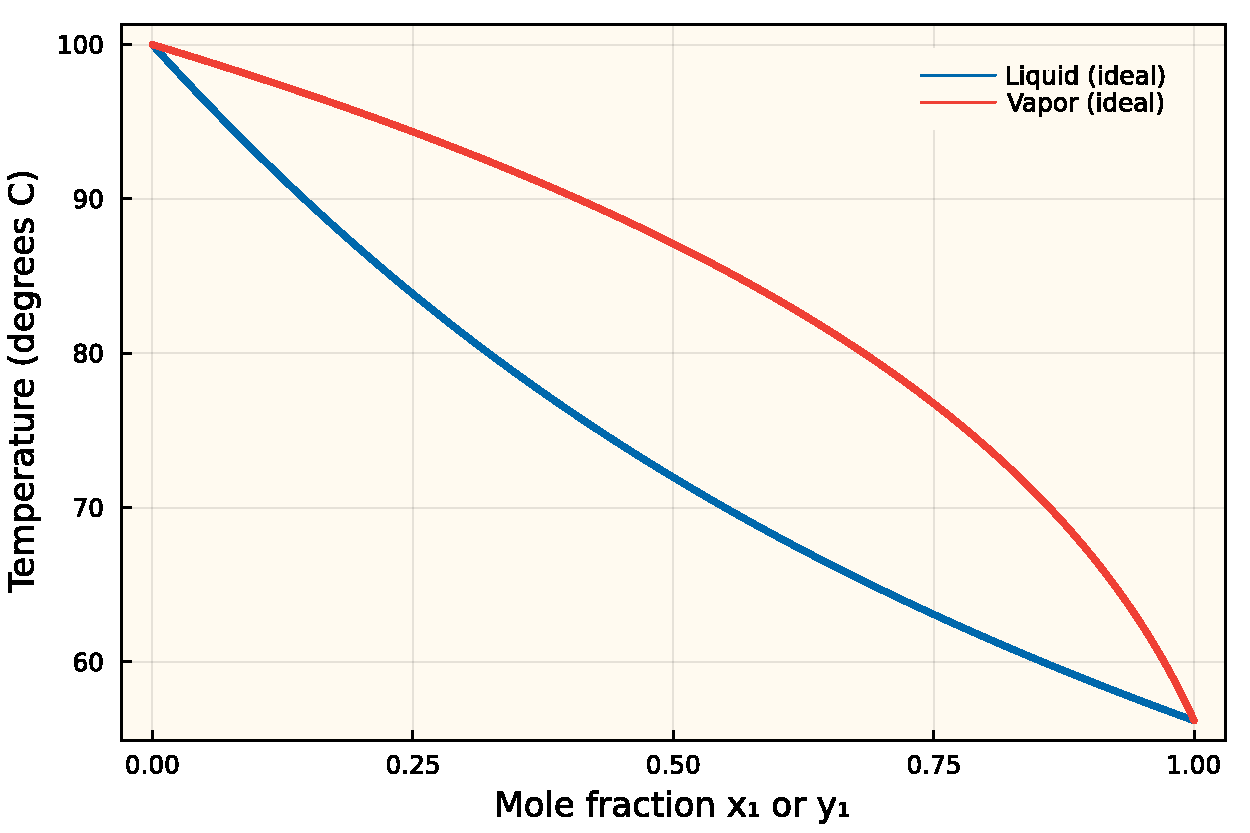
\includegraphics[width=0.75\textwidth]{./figs/Fig-Txy-acetone-water-ideal-P101_325-kPa.pdf}
\caption{Temperature ($^{\circ}C$) versus composition (x$_{1}$ or y$_{1}$) for a binary mixture of Acetone(1)/Water(2) computed assuming ideal liquid and vapor phases.}\label{fig-VLE-ideal-problem-Txy}
\end{figure*}

\item{(XX points)
Cornell Inc. was hired to design a flash separation process for a binary ($\mathcal{M}$ = 2) mixture of Acetone(1)/Water(2).
The engineering team performed initial design calculations assuming an ideal liquid and vapor phase for z$_{1}$ = 0.50
(Fig. \ref{fig-VLE-ideal-problem-Txy}). 

Let the saturation pressure of component $i$ be described by the Antoine equation:
\begin{equation}
  \ln\left(P_{i}^{sat}\right) = A - \frac{B}{C+T}
\end{equation}where $P_{i}^{sat}$ has units of kPa and the temperature $T$ has units of $^{\circ}C$.
The Antoine parameters are given by:

\begin{table}[!ht]
  \centering
  \caption{Antoine parameters for the Acetone/Water flash problem.}
  \setlength{\tabcolsep}{18pt}
  \begin{tabular}{c|c|c|c}\toprule
    Species & A & B & C \\ \toprule
    Acetone & 14.31 & 2756.22 & 228.06 \\
    Water & 16.39 & 3885.7 & 230.17 \\\bottomrule
  \end{tabular}
\end{table}

\textbf{Assumptions}: (i) the Flash drum operates at steady-state;
(ii) vapor-liquid equilibrium occurs everywhere inside the drum at some (T,P);
(iii) treat both the vapor and liquid phases as ideal;
(iv) the Flash drum is well-mixed;
(v) a single liquid feed (stream 1) enters, and a vapor (stream 2) and liquid (stream 3) exit the drum;
(vi) R = 8.314 L kPa K$^{-1}$ mol$^{-1}$.

\begin{itemize}
    \item[a)]{(XX points)~What pressure is the Flash drum operating at? (place your estimated pressure value in Table
    \ref{tbl-state-flash-problem-txy}).}
    \item[b)]{(XX points)~Estimate the missing values in Table \ref{tbl-state-flash-problem-txy} assuming the Flash drum operates at at T = 80$^{\circ}$C with a input feed rate of $\dot{F}$ = 10 mol/t and $z_{1}$ = 0.50.}
  \end{itemize}

  \clearpage

\begin{table}[!ht]
    \centering
    \caption{State table for the Acetone/Water flash problem.}\label{tbl-state-flash-problem-txy}
    \renewcommand{\arraystretch}{2.0}
    \setlength{\tabcolsep}{18pt}
    \begin{tabular}{c|c|c|c|c|c|c}\toprule
    Stream & State & P (kPa) & $\dot{n}_{s,T}$ (mol/t) & $x_{1}$ or $y_{1}$ & $x_{2}$ or $y_{2}$ & T ($^{\circ}$C) \\ \toprule
    1 & L & N/A & 10 & 0.50 &  & N/A \\ \hline
    2 & V & & & & &  \\ \hline
    3 & L & & & & &  \\ \bottomrule
    \end{tabular}
  \end{table}
}
% ================================ %


% Question 4 ===================== %
% \clearpage
% \include{Q1_v1}
% ================================ %

% Extra -
\clearpage

\end{enumerate}

\end{document}
